\documentclass[11pt, a4paper, oneside]{scrreprt}

% --- LINGUA E CODIFICA ---
\usepackage[utf8]{inputenc}
\usepackage[italian]{babel}
\usepackage[margin=2.5cm]{geometry}

% --- PACCHETTI MATEMATICI E FISICI ---
\usepackage{amsmath, amssymb, mathtools}
\usepackage{physics2}
\usepackage{siunitx}
\usepackage{microtype} % Migliora la spaziatura tipografica

% --- GRAFICA E BOX ---
\usepackage{graphicx}
\usepackage{xcolor}
\usepackage[most]{tcolorbox}
\usepackage{subcaption}

% --- NAVIGABILITÀ E HYPERREF ---
\usepackage{hyperref}
\hypersetup{
    colorlinks=true,
    linkcolor=blue!70!black,
    citecolor=green!50!black,
    urlcolor=magenta
}

% --- STILI PERSONALIZZATI PER BOX ---
\newtcolorbox{formulaBox}[1]{
    colback=blue!5!white,
    colframe=blue!75!black,
    fonttitle=\bfseries,
    title=#1,
    arc=2mm
}

\newtcolorbox{notaBox}[1]{
    colback=orange!5!white,
    colframe=orange!85!black,
    fonttitle=\bfseries,
    title=#1,
    arc=2mm
}

% --- INFORMAZIONI DOCUMENTO ---
\title{
    \Huge \textbf{Processi Astrofisici} \\
    \large Appunti del Corso --- Università di Pisa
}
\author{\textbf{Stefano Nordio}}
\date{Anno Accademico 2026/2027}

\begin{document}

\maketitle
\tableofcontents
\newpage

\chapter{Prefazione}
Questi sono i miei appunti riscritti in maniera sensata e leggibile per il corso di Astrophysical Processes
dell'Università di Pisa, tenuto dai professori Crisostomi e Pallottini nell'anno del Signore 2026.
Il corso appare ampio e un po' frammentato, per questo ho ritenuto che fosse utile scrivere
in maniera compatta e organizzata questi appunti, nel modo più coerente a me possibile. Ovviamente le informazioni
riportate potrebbero contenere errori, che vi invito a segnalare alla mia e-mail Unipi.
Il corso è tenuto in inglese, motivo per cui ho scelto di redigere gli appunti in italiano.

% --- CAPITOLO 1 ---
\chapter{L'equazione del Trasporto di Boltzmann}
Questo corso si può riassumere con l'equazione del trasporto di Boltzmann.

\begin{formulaBox}{Equazione del Trasporto di Boltzmann (BTE)}
\begin{equation}
    \frac{df}{dt} = \left. \frac{\partial f}{\partial t} \right|_{\text{coll}}
\end{equation}
dove $f$ è la funzione di distribuzione del sistema di cui vogliamo studiare il comportamento.
\end{formulaBox}

Sul membro di destra di quest'equazione, detto termine collisionale, ci soffermeremo a lungo in più occasioni nel seguito.
Il membro di sinistra della BTE (\textit{Boltzmann Transport Equation}) è la derivata totale rispetto al tempo della funzione di
distribuzione $f(t, \vec{x}, \vec{p})$, la quale dipende dal tempo $t$, dalla posizione $\vec{x}$ e dall'impulso $\vec{p}$.
Essa rappresenta la densità numerica di particelle $N$ nello spazio delle fasi a un determinato istante $t$.
Potrebbe trattarsi, ad esempio, di fotoni, gas, plasma o materia oscura, e ci permette di ottenere una descrizione statistica completa del sistema.

\begin{equation} \label{eq:densita_spazio_fasi}
    f = \frac{d^6N}{dV_x \, dV_p} = \frac{d^6N}{dx \, dy \, dz \, dp_x \, dp_y \, dp_z}
\end{equation}

Proviamo a scrivere il termine di sinistra per una generica funzione $f(t, \vec{x}, \vec{p})$ applicando
la regola di derivazione a catena:

\begin{equation} \label{eq:derivazione_a_catena}
    \frac{df}{dt} = \frac{\partial f}{\partial t} + \dot{\vec{x}} \cdot \vec{\nabla}_{x}f + \dot{\vec{p}} \cdot \vec{\nabla}_{p}f
\end{equation}

Analizziamo i vari termini ottenuti: $\dot{\vec{x}}$ è chiaramente una velocità, mentre $\dot{\vec{p}}$ è una generica forza agente sulla nostra particella.
Siccome la funzione di distribuzione vive nello spazio delle fasi, ci interessa connetterla all'Hamiltoniana del sistema.
Definiamo quindi il vettore $\vec{z}$ nel seguente modo:
\begin{equation}
    \vec{z} = (\vec{x}, \vec{p}) = (x, y, z, p_x, p_y, p_z)
\end{equation}

Allora possiamo riscrivere l'equazione \eqref{eq:derivazione_a_catena} nel seguente modo:
\begin{equation}
    \frac{df}{dt} = \frac{\partial f}{\partial t} + \dot{\vec{z}} \cdot \vec{\nabla}_{z}f
\end{equation}

Ci farebbe comodo riscrivere il secondo termine sfruttando la divergenza del prodotto $(\dot{\vec{z}} f)$.
Usando la regola del prodotto per la divergenza:
\begin{equation}
    \vec{\nabla}_{z} \cdot (\dot{\vec{z}} f) = \dot{\vec{z}} \cdot \vec{\nabla}_{z}f + f \, (\vec{\nabla}_{z} \cdot \dot{\vec{z}})
\end{equation}

da cui ricaviamo:
\begin{equation}
    \frac{df}{dt} = \frac{\partial f}{\partial t} + \dot{\vec{z}} \cdot \vec{\nabla}_{z}f = \frac{\partial f}{\partial t} + \vec{\nabla}_{z} \cdot (\dot{\vec{z}}f) - f \, (\vec{\nabla}_{z} \cdot \dot{\vec{z}})
\end{equation}

A questo punto, la divergenza del campo vettoriale nello spazio delle fasi $\vec{\nabla}_{z} \cdot \dot{\vec{z}}$ vale:
\begin{equation}
    \vec{\nabla}_{z} \cdot \dot{\vec{z}} = \vec{\nabla}_{x} \cdot \dot{\vec{x}} + \vec{\nabla}_{p} \cdot \dot{\vec{p}}
\end{equation}

Sfruttando le equazioni di Hamilton:
\begin{align} \label{eq:proprieta_hamiltoniana}
    \dot{\vec{x}} &= \vec{\nabla}_{p}H \\
    \dot{\vec{p}} &= -\vec{\nabla}_{x}H \nonumber
\end{align}

Otteniamo:
\begin{equation}
    \vec{\nabla}_{z} \cdot \dot{\vec{z}} = \vec{\nabla}_{x} \cdot \vec{\nabla}_{p}H - \vec{\nabla}_{p} \cdot \vec{\nabla}_{x}H = (\vec{\nabla}_{x} \cdot \vec{\nabla}_{p} - \vec{\nabla}_{p} \cdot \vec{\nabla}_{x})H
\end{equation}

Se l'Hamiltoniana è sufficientemente regolare, si ottiene $\vec{\nabla}_{z} \cdot \dot{\vec{z}} = 0$, che esprime l'incomprimibilità del flusso nello spazio delle fasi.

Se poniamo solo per un momento $\left. \frac{\partial f}{\partial t} \right|_{\text{coll}} = 0$, otteniamo l'equazione di Vlasov.
\begin{equation} \label{eq:Vlasov}
    \frac{df}{dt} = \frac{\partial f}{\partial t} + \vec{\nabla}_{z} \cdot (\dot{\vec{z}}f) = 0
\end{equation}

L'equazione \eqref{eq:Vlasov} rappresenta la conservazione della densità di particelle lungo le traiettorie nello spazio delle fasi,
in accordo con il Teorema di Liouville, affrontato nel corso di Meccanica Classica.

Soffermiamoci un attimo a riflettere su cosa comportino le varie componenti della BTE:
\begin{itemize}
    \item Se il flusso nello spazio delle fasi non fosse incomprimibile ($\vec{\nabla}_{z} \cdot \dot{\vec{z}} \neq 0$), significherebbe che sul sistema agiscono forze non-conservative o dissipative (ad esempio forze d'attrito dipendenti dalla velocità).
    \item Se invece la derivata totale non è nulla ($\frac{df}{dt} \neq 0$), significa che il termine collisionale $\left. \frac{\partial f}{\partial t} \right|_{\text{coll}}$ è non nullo a sua volta. In questo caso, processi fisici esterni stanno immettendo o rimuovendo particelle da quel volume infinitesimo dello spazio delle fasi.
    Per esempio, se $f$ rappresenta la funzione di distribuzione dei fotoni di un fascio di luce e questi incontrano un atomo di idrogeno, l'eventuale assorbimento di un fotone da parte dell'atomo verrà descritto proprio all'interno del termine collisionale.
\end{itemize}

\section{Invarianza della BTE}
Prima di applicare l'equazione del trasporto di Boltzmann in ambito astrofisico, è fondamentale verificare che essa sia invariante per cambio di sistema di riferimento inerziale.

Ricordiamo brevemente gli elementi fondamentali della cinematica relativistica.
Nella Figura \ref{fig:confronto_spazi} sono rappresentati graficamente lo spazio-tempo di Minkowski e la relazione di dispersione per una particella massiva di energia $E$ e impulso $\vec{p}$.
Il quadri-vettore posizione $X^\mu$ e il quadri-impulso $P^\mu$ sono definiti come:
\begin{align} \label{eq:relativita}
    X^{\mu} &= (ct, \vec{x}), \quad P^{\mu} = \left(\frac{E}{c}, \vec{p}\right) = (m\gamma c, m\gamma\vec{v}) \\[0.5em]
    P^{\mu}P_{\mu} &= \left(\frac{E}{c}\right)^2 - |\vec{p}|^2 = (mc)^2 \nonumber
\end{align}
dove $\gamma = \frac{1}{\sqrt{1 - \beta^2}}$ è il fattore Lorentziano e $\beta = \frac{v}{c}$.

\begin{figure}[htbp]
    \centering
    \begin{subfigure}[b]{0.48\textwidth}
        \centering
        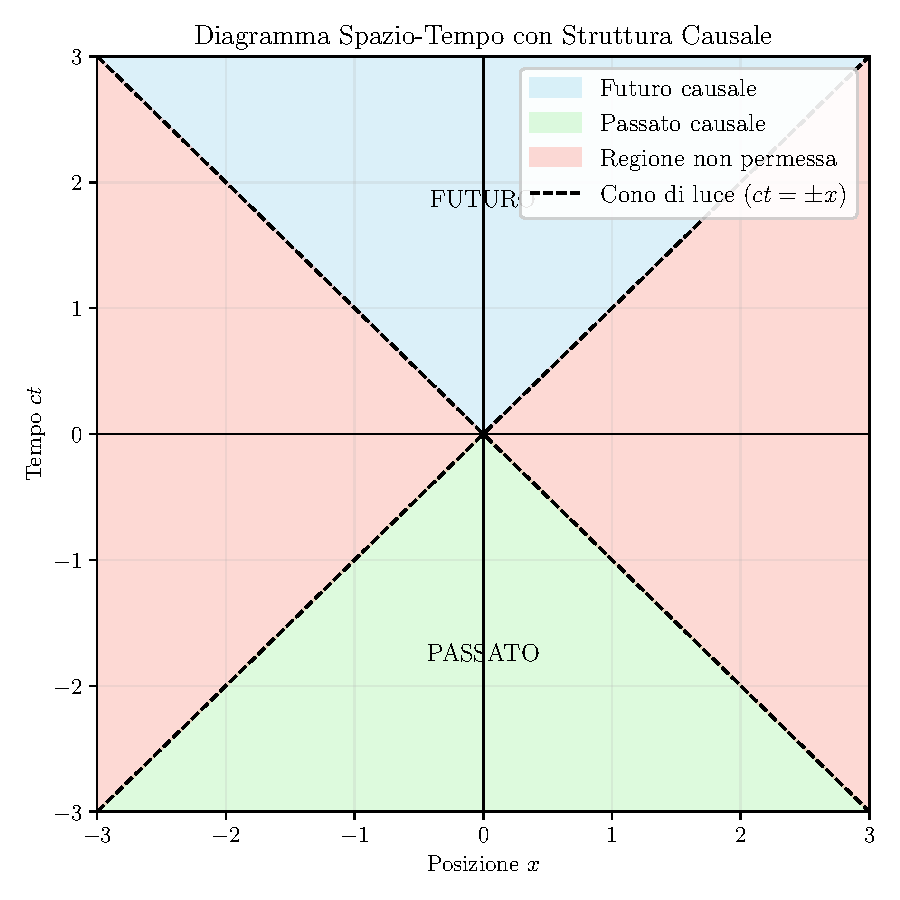
\includegraphics[width=\textwidth]{spazio_tempo_tempo_posizione.pdf}
        \caption{Spazio-tempo di Minkowski.}
        \label{fig:sub_spaziotempo}
    \end{subfigure}
    \hfill
    \begin{subfigure}[b]{0.48\textwidth}
        \centering
        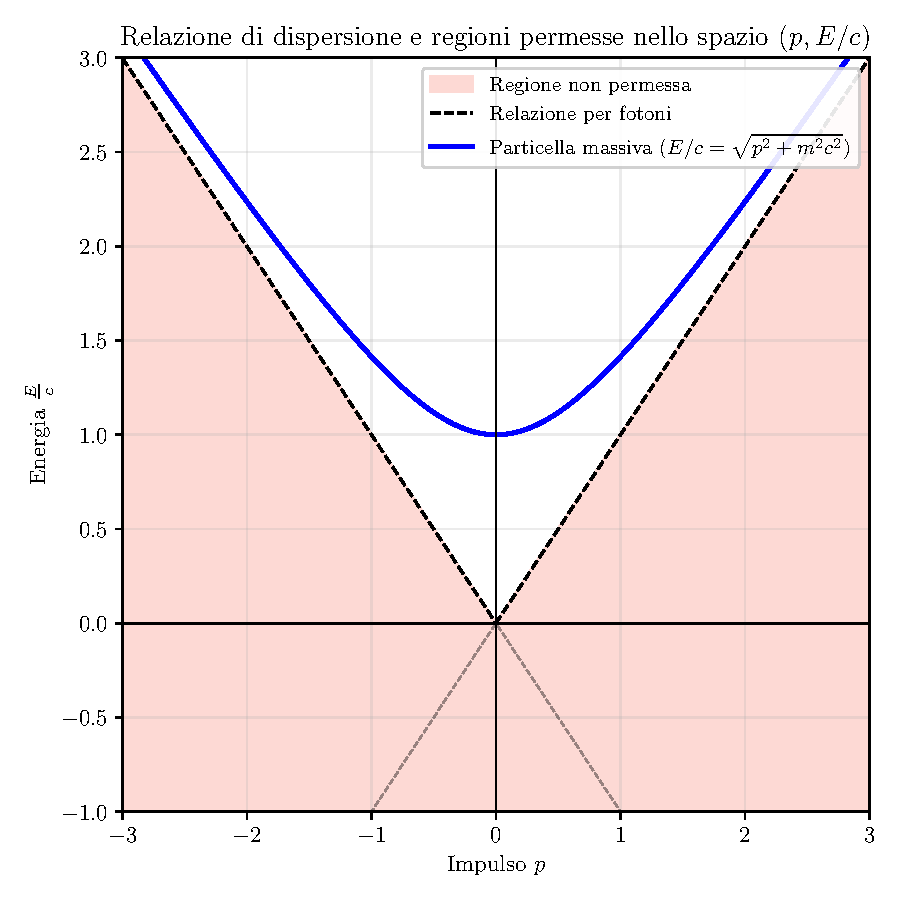
\includegraphics[width=\textwidth]{spazio_tempo_energia_impulso.pdf}
        \caption{Spazio impulso-energia $(p, E/c)$.}
        \label{fig:sub_energia_impulso}
    \end{subfigure}
    \caption{Confronto tra le regioni permesse nello spazio fisico e nello spazio delle fasi.}
    \label{fig:confronto_spazi}
\end{figure}

Consideriamo due sistemi di riferimento inerziali, $S$ e $S'$, in moto relativo con velocità $v$ lungo la direzione dell'asse $x$.
La trasformazione tra le coordinate è descritta dalla matrice di Lorentz $\Lambda_{boost}$:
\begin{equation} \label{eq:boost_x}
    \mathbf{\Lambda}_{\text{boost}} = \begin{pmatrix}
        \gamma & -\beta\gamma & 0 & 0 \\
        -\beta\gamma & \gamma & 0 & 0 \\
        0 & 0 & 1 & 0 \\
        0 & 0 & 0 & 1
    \end{pmatrix}
\end{equation}

Il nostro obiettivo è verificare l'invarianza della funzione di distribuzione nello spazio delle fasi $f(\vec{x}, \vec{p}, t) = \frac{d^6N}{d^3x \, d^3p}$.
Poiché il numero di particelle $dN$ è un conteggio discreto di linee d'universo e costituisce uno scalare di Lorentz ($dN' = dN$), la funzione $f$ sarà invariante se e solo se l'elemento di volume dello spazio delle fasi $d^3x \, d^3p$ è esso stesso invariante di Lorentz.

\subsection*{1. Trasformazione dell'elemento di volume spaziale $d^3x$}

Consideriamo un gruppo di particelle contenute in un elemento di volume $d^3x = dx \, dy \, dz$ nel sistema $S$. Poiché le dimensioni trasversali non sono influenzate dal boost ($dy' = dy$ e $dz' = dz$), si ha $d^3x' = dx' \, dy \, dz$.

Per determinare come si trasforma l'elemento di volume tridimensionale occupato dalle particelle, è necessario considerare il volume proprio$d^3x_0$, ossia il volume misurato nel sistema di riferimento di quiete istantaneo del gruppo di particelle. A causa della contrazione delle lunghezze relativistica, il volume $d^3x$ misurato in un generico sistema $S$ in cui le particelle hanno energia $E = \gamma_{\vec{v}} mc^2$ è legato al volume proprio da:
\begin{equation}
    d^3x = \frac{d^3x_0}{\gamma_{\vec{v}}} = \frac{mc^2}{E} \, d^3x_0 \implies d^3x_0 = \frac{E}{mc^2} \, d^3x
\end{equation}
Essendo il volume proprio $d^3x_0$ e la massa $m$ due invarianti scalari, ne consegue che la combinazione $E \, d^3x$ deve essere un'invariante di Lorentz. Di conseguenza, nel passaggio dal sistema $S$ al sistema $S'$ si ottiene la relazione di trasformazione per il volume spaziale:
\begin{equation} \label{eq:volume_trasformazione}
    d^3x' = \frac{E}{E'} \, d^3x
\end{equation}

\subsection*{2. Trasformazione dell'elemento di volume degli impulsi $d^3p$}

Occupiamoci ora dell'elemento di volume nello spazio degli impulsi $d^3p = dp_x \, dp_y \, dp_z$. Applicando il boost \eqref{eq:boost_x} al quadri-impulso $P^\mu$, otteniamo le componenti trasformate:
\begin{equation} \label{eq:boost_quadrimpulso}
    \begin{pmatrix}
        E'/c \\
        p'_x \\
        p'_y \\
        p'_z
    \end{pmatrix}
    =
    \begin{pmatrix}
        \gamma & -\beta\gamma & 0 & 0 \\
        -\beta\gamma & \gamma & 0 & 0 \\
        0 & 0 & 1 & 0 \\
        0 & 0 & 0 & 1
    \end{pmatrix}
    \begin{pmatrix}
        E/c \\
        p_x \\
        p_y \\
        p_z
    \end{pmatrix}
    =
    \begin{pmatrix}
        \gamma \frac{E}{c} - \beta\gamma p_x \\
        \gamma p_x - \beta\gamma \frac{E}{c} \\
        p_y \\
        p_z
    \end{pmatrix}
\end{equation}
Poiché $p'_y = p_y$ e $p'_z = p_z$, si ha $d^3p' = dp'_x \, dp_y \, dp_z$. Per ricavare il differenziale $dp'_x$, differenziamo l'espressione di $p'_x = \gamma \left( p_x - \frac{v}{c^2} E \right)$:
\begin{equation} \label{eq:diff_px_1}
    dp'_x = \gamma \left( dp_x - \frac{v}{c^2} dE \right)
\end{equation}

Sfruttando la relazione vincolare *on-shell* tra energia e impulso $E^2 = |\vec{p}|^2 c^2 + m^2 c^4$, differenziamo rispetto a $p_x$ tenendo $p_y, p_z$ costanti:
\begin{equation} \label{eq:diff_energia}
    2E \, dE = 2 p_x c^2 \, dp_x \implies dE = \frac{c^2 p_x}{E} \, dp_x
\end{equation}

Sostituendo l'equazione \eqref{eq:diff_energia} nella \eqref{eq:diff_px_1}, raccogliamo il fattore $dp_x$:
\begin{equation}
    dp'_x = \gamma \left( 1 - \frac{v p_x}{E} \right) dp_x
\end{equation}

Dall'espressione dell'energia trasformata $E'$ in \eqref{eq:boost_quadrimpulso}, notiamo che:
\begin{equation}
    E' = \gamma E \left( 1 - \frac{v p_x}{E} \right) \implies \gamma \left( 1 - \frac{v p_x}{E} \right) = \frac{E'}{E}
\end{equation}

Di conseguenza, la relazione tra i differenziali dell'impulso si riduce semplicemente a:
\begin{equation} \label{eq:relazione_differenziali_p}
    dp'_x = \frac{E'}{E} \, dp_x
\end{equation}
e moltiplicando per i differenziali trasversali inalterati ($dp_y dp_z$) otteniamo come varia l'elemento di volume tridimensionale degli impulsi:
\begin{equation}
    d^3p' = \frac{E'}{E} \, d^3p \implies \frac{d^3p'}{E'} = \frac{d^3p}{E}
\end{equation}
Il rapporto $\frac{d^3p}{E}$ costituisce la celebre misura di integrazione invariante di Lorentz nello spazio degli impulsi.

\subsection*{3. Invarianza della funzione di distribuzione}

Combinando la trasformazione dell'elemento di volume spaziale \eqref{eq:volume_trasformazione} e di quello degli impulsi \eqref{eq:relazione_differenziali_p}, calcoliamo la trasformazione dell'elemento di volume totale dello spazio delle fasi $d^6z$:
\begin{equation} \label{eq:invarianza_spazio_fasi}
    d^3x' \, d^3p' = \left( \frac{E}{E'} \, d^3x \right) \left( \frac{E'}{E} \, d^3p \right) = d^3x \, d^3p
\end{equation}

I due fattori scalanti $\frac{E}{E'}$ e $\frac{E'}{E}$ si elidono esattamente. Poiché sia il numero di particelle $dN$ sia l'elemento di volume dello spazio delle fasi $d^3x \, d^3p$ sono invarianti di Lorentz, ne consegue che la funzione di distribuzione del sistema:
\begin{equation}
    f'(\vec{x}', \vec{p}', t') = \frac{dN'}{d^3x' \, d^3p'} = \frac{dN}{d^3x \, d^3p} = f(\vec{x}, \vec{p}, t)
\end{equation}
è uno \textbf{scalare di Lorentz esatto}.
Questo garantisce che la forma dell'equazione del trasporto di Boltzmann rimanga formalmente identica in qualsiasi sistema di riferimento inerziale.

\chapter{Definizioni Fondamentali}
Ci concentriamo per adesso sul trattare fotoni.
Poiché i fotoni non hanno massa, il loro quadrimpulso può essere scritto come:
\begin{equation} \label{quadrimpulso_fotone}
    P^{\mu} = \left(\frac{E}{c}, \vec{p}\right) = \frac{E}{c}\left(1, \frac{\vec{p}c}{E}\right) = \frac{h\nu}{c}(1, \hat{n})
\end{equation}
dove $h$ è la costante di Planck e vale circa $6.626 \cdot 10^{-27}$ erg$\cdot$s.
Prendendo l'equazione \eqref{eq:derivazione_a_catena} e imponendo $p$ costante dato che non siamo in relatività generale, ricaviamo:
\begin{equation} \label{eq:Boltzmann_fotoni}
    \frac{df_{\gamma}(t, \vec{x}, \nu, \hat{n})}{dt} = \frac{\partial f_{\gamma}}{\partial t} + c\hat{n} \cdot \vec{\nabla}_{x}f_{\gamma}
\end{equation} 

\section{L'intensità specifica monocromatica}
Definiamo, quindi, l'\textbf{intensità specifica monocromatica} come:

\begin{formulaBox}{Intensità specifica monocromatica}
\begin{equation} \label{eq:intensita_specifica_monocromatica}
    I_{\nu} = \frac{dE_\nu}{dA \, d\Omega \, dt \, d\nu}
\end{equation}
dove $dE_\nu$ è il differenziale dell'energia a una data frequenza, $dA$ l'elemento d'area infinitesimo attraversato dai fotoni, $d\Omega$ l'elemento infinitesimo di angolo solido e $\nu$ la frequenza. 
\end{formulaBox}

Si tratta di una potenza per unità d'area, di angolo solido e frequenza, la cui unità di misura è $\frac{\text{erg}}{\text{cm}^2 \cdot \text{sr} \cdot \text{Hz} \cdot \text{s}}$ nel sistema CGS.
Questa grandezza macroscopica è direttamente collegata alla funzione di distribuzione microscopica $f_{\gamma}$ dello spazio delle fasi.
Cerchiamo, perciò, una relazione tra l'intensità specifica monocromatica e la distribuzione di probabilità, analizzando nuovamente l'elemento infinitesimo di volume dello spazio delle fasi.
\begin{equation} \label{eq:pre_normalizzazione}
    dN_{\gamma} = f_{\gamma}(I_{\nu}) \, dV_x \, dV_p, \quad \text{con} \quad N_{\gamma}(t) = \int_{V_x} \int_{V_p} f_{\gamma}(t, \vec{x}, \vec{p}) \, d^3x \, d^3p
\end{equation}

Ci accorgiamo che l'elemento di volume $dV_x$ attraversato dai fotoni in un tempo $dt$ è:
\begin{equation} \label{eq:volume_fotoni}
    dV_x = c \, dA \, dt
\end{equation}
Inoltre, possiamo riscrivere l'elemento di volume $dV_p$ in coordinate sferiche:
\begin{equation} \label{eq:vp_sferiche}
    dV_p = dp_x \, dp_y \, dp_z = p^2 \, dp \, d(\cos\theta) \, d\phi = p^2 \, dp \, d\Omega
\end{equation}

Sostituendo nell'equazione \eqref{eq:vp_sferiche} la relazione $p = \frac{h\nu}{c}$ e $dp = \frac{h}{c} d\nu$ otteniamo:
\begin{equation} \label{eq:vp_fotoni}
    dV_p = \left(\frac{h}{c}\right)^3 \, \nu^2 \, d\nu \, d\Omega
\end{equation}

Cambiamo la normalizzazione dell'equazione \eqref{eq:pre_normalizzazione}:
\begin{equation} \label{eq:pre_normalizzazione_2}
    dN_{\gamma} = f_{\gamma}(I_{\nu}) \, dV_x \, dV_p = 2 n_{\gamma} \frac{dV_x \, dV_p}{h^3}
\end{equation}
dove $n_{\gamma}$ è il numero di occupazione dei fotoni e $2$ la degenerazione dovuta alle due possibili polarizzazioni.
Possiamo, quindi, sostituire nell'equazione \eqref{eq:intensita_specifica_monocromatica} le equazioni \eqref{eq:pre_normalizzazione_2}, \eqref{eq:volume_fotoni} e \eqref{eq:vp_fotoni}, sapendo che $dE_{\nu} = h\nu \, dN_{\gamma}$:
\begin{align}
    I_{\nu} &= \frac{dE_\nu}{dA \, d\Omega \, dt \, d\nu} = \frac{h\nu \, dN_{\gamma}}{dA \, d\Omega \, dt \, d\nu} \nonumber \\[0.5em]
    &= \frac{h\nu}{dA \, d\Omega \, dt \, d\nu} \left[ \frac{2 n_{\gamma}}{h^3} \left(c \, dA \, dt\right) \left( \frac{h^3}{c^3} \nu^2 \, d\nu \, d\Omega \right) \right] \nonumber \\[0.5em]
    &= \frac{2 h \nu^3}{c^2} n_{\gamma}
\end{align}





\end{document}